%%%%%%%%%%%%%%%%%%%%%%%%%%%%%%%%%%%%%%%%%%%%%%%%%%%%%%%%%%%%%%%%%%%%%%%%%%%%%%%%
% Template for USENIX papers.
%
% History:
%
% - TEMPLATE for Usenix papers, specifically to meet requirements of
%   USENIX '05. originally a template for producing IEEE-format
%   articles using LaTeX. written by Matthew Ward, CS Department,
%   Worcester Polytechnic Institute. adapted by David Beazley for his
%   excellent SWIG paper in Proceedings, Tcl 96. turned into a
%   smartass generic template by De Clarke, with thanks to both the
%   above pioneers. Use at your own risk. Complaints to /dev/null.
%   Make it two column with no page numbering, default is 10 point.
%
% - Munged by Fred Douglis <douglis@research.att.com> 10/97 to
%   separate the .sty file from the LaTeX source template, so that
%   people can more easily include the .sty file into an existing
%   document. Also changed to more closely follow the style guidelines
%   as represented by the Word sample file.
%
% - Note that since 2010, USENIX does not require endnotes. If you
%   want foot of page notes, don't include the endnotes package in the
%   usepackage command, below.
% - This version uses the latex2e styles, not the very ancient 2.09
%   stuff.
%
% - Updated July 2018: Text block size changed from 6.5" to 7"
%
% - Updated Dec 2018 for ATC'19:
%
%   * Revised text to pass HotCRP's auto-formatting check, with
%     hotcrp.settings.submission_form.body_font_size=10pt, and
%     hotcrp.settings.submission_form.line_height=12pt
%
%   * Switched from \endnote-s to \footnote-s to match Usenix's policy.
%
%   * \section* => \begin{abstract} ... \end{abstract}
%
%   * Make template self-contained in terms of bibtex entires, to allow
%     this file to be compiled. (And changing refs style to 'plain'.)
%
%   * Make template self-contained in terms of figures, to
%     allow this file to be compiled. 
%
%   * Added packages for hyperref, embedding fonts, and improving
%     appearance.
%   
%   * Removed outdated text.
%
%%%%%%%%%%%%%%%%%%%%%%%%%%%%%%%%%%%%%%%%%%%%%%%%%%%%%%%%%%%%%%%%%%%%%%%%%%%%%%%%

\documentclass[letterpaper,twocolumn,10pt]{article}
\usepackage{usenix-2020-09}
\usepackage{subfiles}
\usepackage{booktabs}


% to be able to draw some self-contained figs
\usepackage{tikz}
\usepackage{amsmath}

% inlined bib file
\usepackage{filecontents}

%-------------------------------------------------------------------------------
\begin{filecontents}{\jobname.bib}
%-------------------------------------------------------------------------------
@misc{ebpf,
  key = {eBPF}
  title =        {Linux Socket Filtering aka Berkeley Packet Filter (BPF)},
  howpublished =         {\url{https://www.kernel.org/doc/Documentation/networking/filter.txt}}
  note = {Accessed: 2024-12-08}
}
@inproceedings{ccp,
    title={Restructuring endpoint congestion control},
    ISBN={9781450355674},
    url={https://dl.acm.org/doi/10.1145/3230543.3230553},
    DOI={10.1145/3230543.3230553},
    booktitle={SIGCOMM},
    author={Narayan, Akshay and Cangialosi, Frank and Raghavan, Deepti and Goyal, Prateesh and Narayana, Srinivas and Mittal, Radhika and Alizadeh, Mohammad and Balakrishnan, Hari},
    year={2018},
}
@inproceedings{ebpf_cca,
author = {Hinz, J\"{o}rn-Thorben and Addanki, Vamsi and Gy\"{o}rgyi, Csaba and Jepsen, Theo and Schmid, Stefan},
title = {TCP's Third Eye: Leveraging eBPF for Telemetry-Powered Congestion Control},
year = {2023},
isbn = {9798400702938},
publisher = {Association for Computing Machinery},
url = {https://doi.org/10.1145/3609021.3609295},
doi = {10.1145/3609021.3609295},
booktitle = {Proceedings of the 1st Workshop on EBPF and Kernel Extensions},
series = {eBPF '23}
}
@inproceedings{CCAStarvation,
author = {Arun, Venkat and Alizadeh, Mohammad and Balakrishnan, Hari},
title = {Starvation in end-to-end congestion control},
year = {2022},
isbn = {9781450394208},
publisher = {Association for Computing Machinery},
address = {New York, NY, USA},
url = {https://doi.org/10.1145/3544216.3544223},
doi = {10.1145/3544216.3544223},
abstract = {To overcome weaknesses in traditional loss-based congestion control algorithms (CCAs), researchers have developed and deployed several delay-bounding CCAs that achieve high utilization without bloating delays (e.g., Vegas, FAST, BBR, PCC, Copa, etc.). When run on a path with a fixed bottleneck rate, these CCAs converge to a small delay range in equilibrium. This paper proves a surprising result: although designed to achieve reasonable inter-flow fairness, current methods to develop delay-bounding CCAs cannot always avoid starvation, an extreme form of unfairness. Starvation may occur when such a CCA runs on paths where non-congestive network delay variations due to real-world factors such as ACK aggregation and end-host scheduling exceed double the delay range that the CCA converges to in equilibrium. We provide experimental evidence for this result for BBR, PCC Vivace, and Copa with a link emulator. We discuss the implications of this result and posit that to guarantee no starvation an efficient delay-bounding CCA should design for a certain amount of non-congestive jitter and ensure that its equilibrium delay oscillations are at least one-half of this jitter.},
booktitle = {Proceedings of the ACM SIGCOMM 2022 Conference},
pages = {177–192},
numpages = {16},
keywords = {starvation, delay-convergence, congestion control},
location = {Amsterdam, Netherlands},
series = {SIGCOMM '22}
}
@INPROCEEDINGS{CCA-Fairness,
  author={Ling, Yang and Xiao-fan, Zhang and Yu-shan, Liu},
  booktitle={2009 International Conference on Wireless Communications & Signal Processing}, 
  title={Analyzing and improving the TCP flow fairness in 802.11 based ad hoc networks}, 
  year={2009},
  volume={},
  number={},
  pages={1-5},
  keywords={Ad hoc networks;Spread spectrum communication;Information science;Information analysis;Costs;Monopoly;Aggregates;Throughput;Media Access Protocol;Quantization;Ad Hoc networks;IEEE 802.11 DCF;TCP flow fairness;Probability model},
  doi={10.1109/WCSP.2009.5371583}}

@inproceedings{CCA-FCC,
author = {Che, Biyao and Wang, Yuxiang and Wan, Zirui and Chen, Ying and Wang, Zixiao and Tian, Yuan and Zhao, Jizhuang and Wang, Shuo and Zhang, Jiao},
title = {FCC : A Fast-Converging Low-Latency Congestion Control Algorithm for Datacenter RDMA Network},
year = {2024},
isbn = {9798400717581},
publisher = {Association for Computing Machinery},
address = {New York, NY, USA},
url = {https://doi.org/10.1145/3663408.3665834},
doi = {10.1145/3663408.3665834},
abstract = {Congestion control plays a crucial role in ensuring the performance of data center networks. However, mainstream RDMA congestion control algorithms still face challenges such as slow congestion response and poor deployability. In this paper, we propose a novel fast-convergence congestion control algorithm, FCC, to address these shortcomings. FCC leverages Explicit Congestion Notification (ECN) and Round-Trip Time (RTT) signals, utilizing the gradient of RTT to enhance response speed and employing a Sigmoid curve for rate increment. Through experiments, we demonstrate that compared to existing state-of-the-art algorithms, FCC achieves superior performance in terms of convergence speed, fairness, and small flow latency metrics.},
booktitle = {Proceedings of the 8th Asia-Pacific Workshop on Networking},
pages = {200–201},
numpages = {2},
keywords = {ECN, RDMA congestion control, RTT, Sigmoid-AI.},
location = {Sydney, Australia},
series = {APNet '24}
}
@article{CCA-BBR,
author = {Cardwell, Neal and Cheng, Yuchung and Gunn, C. Stephen and Yeganeh, Soheil Hassas and Jacobson, Van},
title = {BBR: Congestion-Based Congestion Control: Measuring bottleneck bandwidth and round-trip propagation time},
year = {2016},
issue_date = {September-October 2016},
publisher = {Association for Computing Machinery},
address = {New York, NY, USA},
volume = {14},
number = {5},
issn = {1542-7730},
url = {https://doi.org/10.1145/3012426.3022184},
doi = {10.1145/3012426.3022184},
abstract = {When bottleneck buffers are large, loss-based congestion control keeps them full, causing bufferbloat. When bottleneck buffers are small, loss-based congestion control misinterprets loss as a signal of congestion, leading to low throughput. Fixing these problems requires an alternative to loss-based congestion control. Finding this alternative requires an understanding of where and how network congestion originates.},
journal = {Queue},
month = oct,
pages = {20–53},
numpages = {34}
}
@inproceedings{PrinciplesForCongestionManagement,
author = {Brown, Lloyd and Alcoz, Albert Gran and Cangialosi, Frank and Narayan, Akshay and Alizadeh, Mohammad and Balakrishnan, Hari and Friedman, Eric and Katz-Bassett, Ethan and Krishnamurthy, Arvind and Schapira, Michael and Shenker, Scott},
title = {Principles for Internet Congestion Management},
year = {2024},
isbn = {9798400706141},
publisher = {Association for Computing Machinery},
address = {New York, NY, USA},
url = {https://doi.org/10.1145/3651890.3672247},
doi = {10.1145/3651890.3672247},
abstract = {Given the technical flaws with---and the increasing non-observance of---the TCP-friendliness paradigm, we must rethink how the Internet should manage bandwidth allocation. We explore this question from first principles, but remain within the constraints of the Internet's current architecture and commercial arrangements. We propose a new framework, Recursive Congestion Shares (RCS), that provides bandwidth allocations independent of which congestion control algorithms flows use but consistent with the Internet's economics. We show that RCS achieves this goal using game-theoretic calculations and simulations as well as network emulation.},
booktitle = {Proceedings of the ACM SIGCOMM 2024 Conference},
pages = {166–180},
numpages = {15},
keywords = {network architecture},
location = {Sydney, NSW, Australia},
series = {ACM SIGCOMM '24}
}
@article{Dismantling,
author = {Briscoe, Bob},
title = {Flow rate fairness: dismantling a religion},
year = {2007},
issue_date = {April 2007},
publisher = {Association for Computing Machinery},
address = {New York, NY, USA},
volume = {37},
number = {2},
issn = {0146-4833},
url = {https://doi.org/10.1145/1232919.1232926},
doi = {10.1145/1232919.1232926},
abstract = {Resource allocation and accountability keep reappearing on every list of requirements for the Internet architecture. The reason we never resolve these issues is a broken idea of what the problem is. The applied research and standards communities are using completely unrealistic and impractical fairness criteria. The resulting mechanisms don't even allocate the right thing and they don't allocate it between the right entities. We explain as bluntly as we can that thinking about fairness mechanisms like TCP in terms of sharing out flow rates has no intellectual heritage from any concept of fairness in philosophy or social science, or indeed real life. Comparing flow rates should never again be used for claims of fairness in production networks. Instead, we should judge fairness mechanisms on how they share out the 'cost' of each user's actions on others},
journal = {SIGCOMM Comput. Commun. Rev.},
month = mar,
pages = {63–74},
numpages = {12},
keywords = {resource allocation, identity, fairness, congestion control, accountability}
}
@misc{iperf,
  author = {The iPerf team},
  title =        {iPerf - The ultimate speed test tool for TCP, UDP and SCTP},
  howpublished =         {\url{https://iperf.fr/}}
  notenote = {Accessed: 2024-11-12}
}
@misc{generic-cong-avoid,
  author = {The CCP Project},
  title =        {CCP Algorithm: Generic Congestion Avoidance},
  howpublished =         {\url{https://github.com/ccp-project/generic-cong-avoid}}
  note = {Accessed: 2024-11-12}
}
\end{filecontents}

%-------------------------------------------------------------------------------
\begin{document}
%-------------------------------------------------------------------------------

%don't want date printed
\date{}

% make title bold and 14 pt font (Latex default is non-bold, 16 pt)
\title{\Large \bf Evaluating eBPF as a Platform for Congestion Control Algorithm}

%for single author (just remove % characters)
\author{
{\rm Edward Wibowo}\\
Brown University
\and
{\rm Bokai Bi}\\
Brown University
% copy the following lines to add more authors
% \and
% {\rm Name}\\
%Name Institution
} % end author

\maketitle

%-------------------------------------------------------------------------------
\begin{abstract}
%-------------------------------------------------------------------------------
\subfile{sections/abstract}
\end{abstract}


%-------------------------------------------------------------------------------
\section{Introduction}
%-------------------------------------------------------------------------------
\subfile{sections/introduction}

%-------------------------------------------------------------------------------
\section{Related Work}
%-------------------------------------------------------------------------------
\subfile{sections/relatedwork}

%-------------------------------------------------------------------------------
\section{Design Overview}
%-------------------------------------------------------------------------------
\subfile{sections/design}

%-------------------------------------------------------------------------------
\section{Evaluation}
%-------------------------------------------------------------------------------
\subfile{sections/evaluation}

%-------------------------------------------------------------------------------
\section{Limitations}
%-------------------------------------------------------------------------------
\subfile{sections/limitations}

%-------------------------------------------------------------------------------
\section{Conclusion}
%-------------------------------------------------------------------------------
\subfile{sections/conclusion}


%% ANYTHING BELOW HERE IS FROM THE ORIGINAL TEMPLATE, SHOULD BE REMOVED LATER

%-------------------------------------------------------------------------------
\section{Footnotes, Verbatim, and Citations}
%-------------------------------------------------------------------------------

Footnotes should be places after punctuation characters, without any
spaces between said characters and footnotes, like so.%
\footnote{Remember that USENIX format stopped using endnotes and is
  now using regular footnotes.} And some embedded literal code may
look as follows.

\begin{verbatim}
int main(int argc, char *argv[]) 
{
    return 0;
}
\end{verbatim}

Now we're going to cite somebody. Watch for the cite tag. Here it
comes. Arpachi-Dusseau and Arpachi-Dusseau co-authored an excellent OS
book, which is also really funny~\cite{arpachiDusseau18:osbook}, and
Waldspurger got into the SIGOPS hall-of-fame due to his seminal paper
about resource management in the ESX hypervisor~\cite{waldspurger02}.

The tilde character (\~{}) in the tex source means a non-breaking
space. This way, your reference will always be attached to the word
that preceded it, instead of going to the next line.

And the 'cite' package sorts your citations by their numerical order
of the corresponding references at the end of the paper, ridding you
from the need to notice that, e.g, ``Waldspurger'' appears after
``Arpachi-Dusseau'' when sorting references
alphabetically~\cite{waldspurger02,arpachiDusseau18:osbook}. 

It'd be nice and thoughtful of you to include a suitable link in each
and every bibtex entry that you use in your submission, to allow
reviewers (and other readers) to easily get to the cited work, as is
done in all entries found in the References section of this document.

Now we're going take a look at Section~\ref{sec:figs}, but not before
observing that refs to sections and citations and such are colored and
clickable in the PDF because of the packages we've included.

%-------------------------------------------------------------------------------
\section{Floating Figures and Lists}
\label{sec:figs}
%-------------------------------------------------------------------------------


%---------------------------
\begin{figure}
\begin{center}
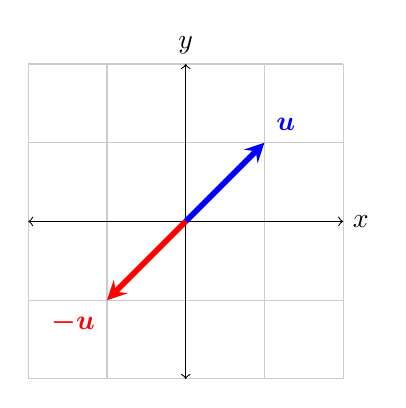
\begin{tikzpicture}
  \draw[thin,gray!40] (-2,-2) grid (2,2);
  \draw[<->] (-2,0)--(2,0) node[right]{$x$};
  \draw[<->] (0,-2)--(0,2) node[above]{$y$};
  \draw[line width=2pt,blue,-stealth](0,0)--(1,1)
        node[anchor=south west]{$\boldsymbol{u}$};
  \draw[line width=2pt,red,-stealth](0,0)--(-1,-1)
        node[anchor=north east]{$\boldsymbol{-u}$};
\end{tikzpicture}
\end{center}
\caption{\label{fig:vectors} Text size inside figure should be as big as
  caption's text. Text size inside figure should be as big as
  caption's text. Text size inside figure should be as big as
  caption's text. Text size inside figure should be as big as
  caption's text. Text size inside figure should be as big as
  caption's text. }
\end{figure}
%% %---------------------------


Here's a typical reference to a floating figure:
Figure~\ref{fig:vectors}. Floats should usually be placed where latex
wants then. Figure\ref{fig:vectors} is centered, and has a caption
that instructs you to make sure that the size of the text within the
figures that you use is as big as (or bigger than) the size of the
text in the caption of the figures. Please do. Really.

In our case, we've explicitly drawn the figure inlined in latex, to
allow this tex file to cleanly compile. But usually, your figures will
reside in some file.pdf, and you'd include them in your document
with, say, \textbackslash{}includegraphics.

Lists are sometimes quite handy. If you want to itemize things, feel
free:

\begin{description}
  
\item[fread] a function that reads from a \texttt{stream} into the
  array \texttt{ptr} at most \texttt{nobj} objects of size
  \texttt{size}, returning returns the number of objects read.

\item[Fred] a person's name, e.g., there once was a dude named Fred
  who separated usenix.sty from this file to allow for easy
  inclusion.
\end{description}

\noindent
The noindent at the start of this paragraph in its tex version makes
it clear that it's a continuation of the preceding paragraph, as
opposed to a new paragraph in its own right.


\subsection{LaTeX-ing Your TeX File}
%-----------------------------------

People often use \texttt{pdflatex} these days for creating pdf-s from
tex files via the shell. And \texttt{bibtex}, of course. Works for us.

%-------------------------------------------------------------------------------
\section*{Acknowledgments}
%-------------------------------------------------------------------------------

The USENIX latex style is old and very tired, which is why
there's no \textbackslash{}acks command for you to use when
acknowledging. Sorry.

%-------------------------------------------------------------------------------
\section*{Availability}
%-------------------------------------------------------------------------------

USENIX program committees give extra points to submissions that are
backed by artifacts that are publicly available. If you made your code
or data available, it's worth mentioning this fact in a dedicated
section.

%-------------------------------------------------------------------------------
\bibliographystyle{plain}
\bibliography{\jobname}

%%%%%%%%%%%%%%%%%%%%%%%%%%%%%%%%%%%%%%%%%%%%%%%%%%%%%%%%%%%%%%%%%%%%%%%%%%%%%%%%
\end{document}
%%%%%%%%%%%%%%%%%%%%%%%%%%%%%%%%%%%%%%%%%%%%%%%%%%%%%%%%%%%%%%%%%%%%%%%%%%%%%%%%

%%  LocalWords:  endnotes includegraphics fread ptr nobj noindent
%%  LocalWords:  pdflatex acks
